\chapter{Estatística bivariada}

Na análise de bancos de dados geralmente se torna necessário comparar duas populações diferentes. Em um depósito mineral, por exemplo, podemos ter diversas variáveis presentes. Em alguns casos a relação entre elas pode ser um indício dos fenômenos genéticos de formação das rochas. Em outros casos apenas estamos interessados em como uma informação secundária pode estar relacionada com uma primária de interesse. Seria proveitoso para nós, por exemplo, traçar um modelo que definisse a chance de obter uma amostra com certo teor em contrapartida de outra amostra com o teor de uma variável diferente. Em um depósito vulcanogênico sulfetado podemos estar interessados em prever a quantidade de um elemento metálico a partir do enxofre da rocha encaixante. Enfim, toda a informação que relaciona duas variáveis pode ser descrita pela estatística bivariada.  

Diferentemente da estatística univariada, a comparação de histogramas de variáveis diferentes não é uma alternativa interessante sobre o ponto de vista prático. É muito difícil determinar a relação entre duas amostras simplesmente pelas suas proporções individuais. Para isso definimos algumas ferramentas que facilitam ao modelador entender a relação entre duas variáveis distintas visualmente e numericamente. 

As seções que se prosseguem mostrarão algumas das ferramentas utilizadas para se caracterizar distribuições bivariadas. 

\section{Gráfico Q-Q plot}

O gráfico q-q plot é uma ferramenta para uma primeira análise de diferentes distribuições de variáveis aleatórias. A Figura \ref{QQplot} demonstra o gráfico q-q plot das variáveis Cobalto e Cádmio.

\begin{figure}[H]
	\centering
	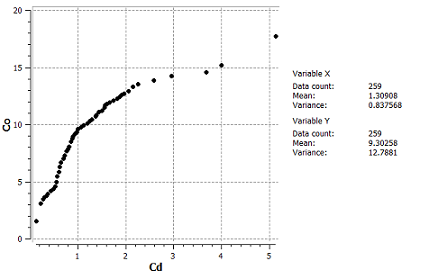
\includegraphics[scale=0.8]{qq-plot.png}	
	\caption{Gráfico QQ-Plot de Cobalto e Cádmio. Nota-se uma curvatura característica demonstrando pequena correspondência entre as duas populações. Cada ponto representa o mesmo percentil para cada variável }
	\label{QQplot}
\end{figure}

Neste gráfico são plotados em cada eixo, para um mesmo percentual acumulado das variáveis aleatórias, os valores dos percentis das variáveis. Distribuições idênticas são representadas por uma reta de 45 graus de inclinação no eixo vertical. Distribuições de variáveis com mesma distribuição mas momentos estatísticos diferentes apresentam comportamento linear, mas inclinações diferentes. 

\section{Gráfico p-p plot}

Semelhante ao gráfico q-q plot temos o gráfico p-p plot. A figura \ref{ppplot} demonstra o gráfico da variável Cobre pela de Cromo. 

\begin{figure}[H]
	\centering
	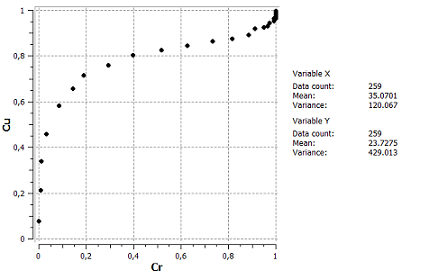
\includegraphics[scale=0.8]{pp-plot.png}	
	\caption{Gráfico PP-Plot de Cobre e Cromo. Nota-se uma curvatura característica demonstrando pouca correspondência entre as duas populações. Cada ponto representa o percentual acumulado para o mesmo valor da variável aleatória }
	\label{ppplot}
\end{figure} 

A análise do gráfico é feita de forma semelhante ao QQ-plot, no entanto, este gráfico é muito mais sensível à mudança de escala das variáveis. Ele é mais vantajoso quando a ordem de grandeza das variáveis analisadas for semelhante. Neste caso estamos comparando a relação de percentuais acumulados diferentes para o mesmo valor da variável aleatória. 

  \section{Gráfico de dispersão}
  
O gráfico de dispersão apresenta dados de duas variáveis dispostos nos eixos cartesianos. Para a utilização do gráfico os dados devem estar colocados. Isso significa que a amostra 1 deve ter a mesma origem da amostra 2, ou o mesmo suporte. Logo só podemos realizar um gráfico de dispersão com vetores de amostras do mesmo tamanho. 

Caso a amostragem apresente dados inválidos para uma variável devemos utilizar um filtro para separar apenas os dados colocados. Existem técnicas estatísticas que permitem o tratamento de dados perdidos ou inexistentes, mas nada substitui a amostra em termos de informação sobre o objeto de estudo. A figura \eqref{scatter} demonstra um gráfico de dispersão entre a variável cromo e cobalto.
  
\begin{figure}[H]
  	\centering
  	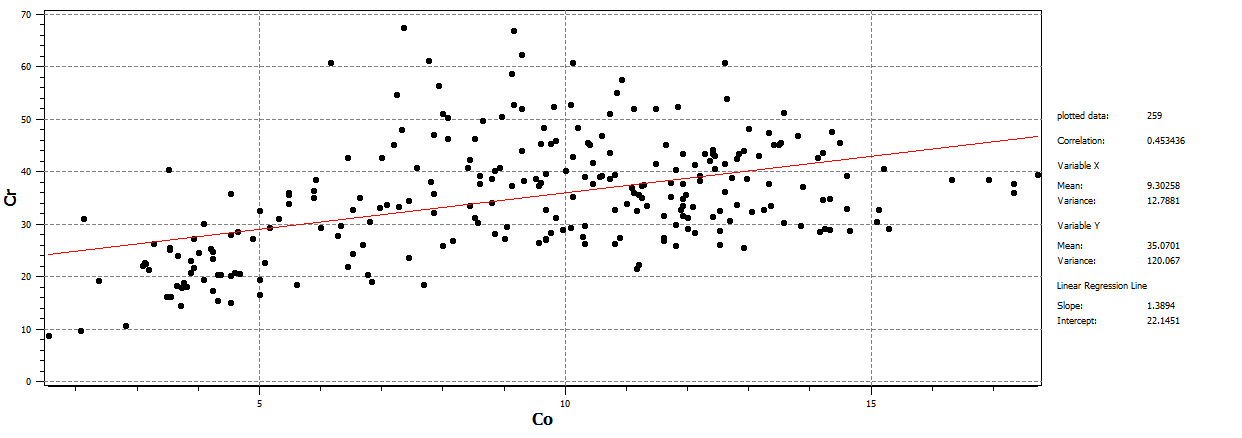
\includegraphics[scale=0.8]{scatter.png}	
  	\caption{Gráfico de dispersão da variável Cromo e Cobalto. Nota-se dependência linear positiva entre as variáveis. }
  	\label{scatter}
\end{figure} 
   
Nota-se pela figura que as variáveis possuem dependência linear positiva entre a variável Cromo e Cobalto. Isso significa que amostras com valor grande de cromo podem apresentar valores grandes de cobalto. 

O contrário também pode acontecer, alguns minerais como quartzo e piroxênio são inversamente proporcionais em rochas magmáticas. À medida em que se aumenta o teor de quartzo tende-se a reduzir o teor de piroxênio na amostra de rocha. 

A Figura \eqref{correlacao_linear} demonstra os tipos de correlação lineares possíveis. Em \eqref{correlacao_linear}a) temos a correlação linear positiva em que o aumento da variável X aumenta o valor de Y, em \eqref{correlacao_linear}b) temos a correlação linear negativa em que o aumento do valor X tende a diminuir o valor de Y e em \eqref{correlacao_linear} temos um caso de independência entre as variáveis, tal que o aumento da variável X não altera o valor da variável Y. 

\begin{figure}[H]
	\centering
	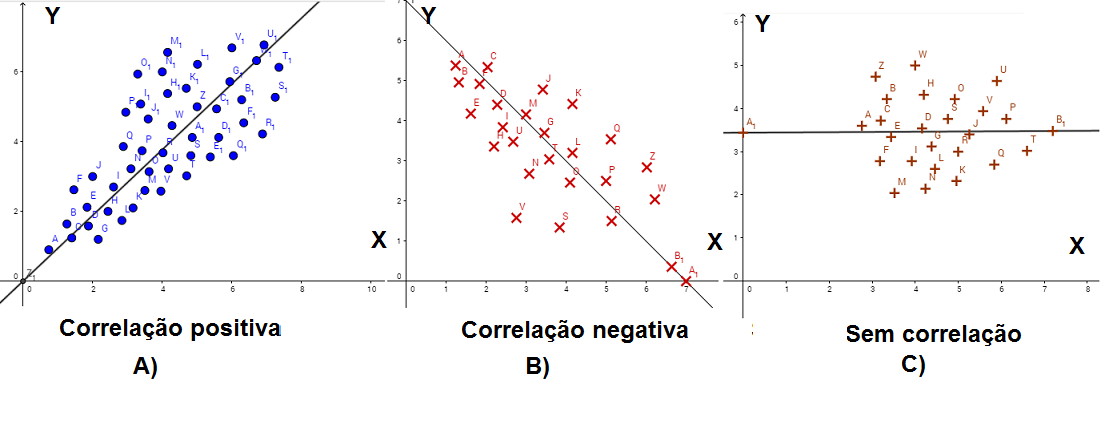
\includegraphics[scale=0.40]{correlacao_linha.png}	
	\caption{Figura demonstrando os tipos de correlação linear possíveis. A) Correlação linear positiva, B) Correlação linear negativa, C) Sem correlação }
	\label{correlacao_linear}
\end{figure}

   
Os gráficos de dispersão também são uma boa medida para a visualização de valores outliers. A figura \eqref{scatter_out} demonstra a dispersão anterior mas com uma área circulada de pontos que não estão dentro do comportamento linear das variáveis. Neste caso para valores intermediários de Cobalto temos grandes valores de Cromo.

 \begin{figure}[H]
 	\centering
 	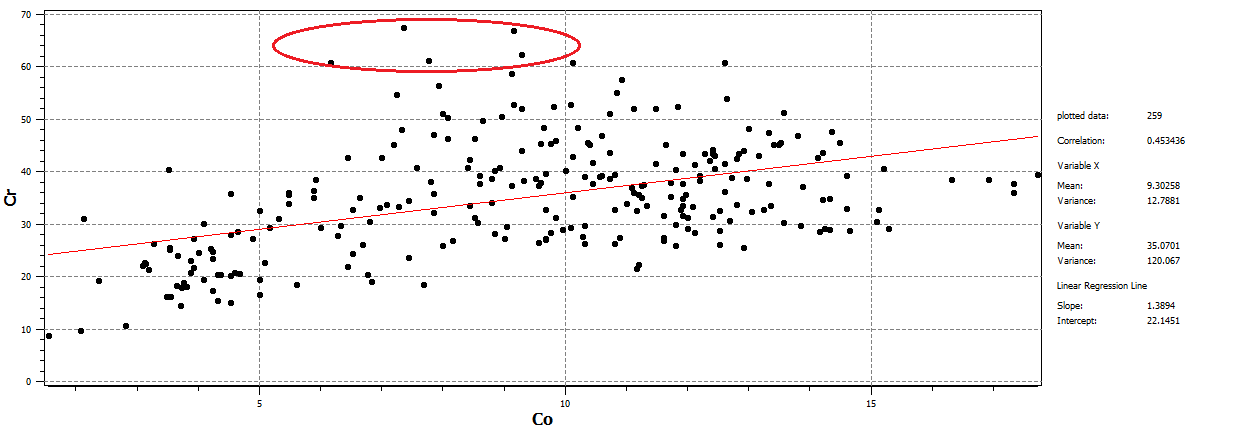
\includegraphics[scale=0.8]{scatter_out.png}	
 	\caption{Gráfico de dispersão da variável Cromo e Cobalto demonstrando valores outliers. Círculo vermelho indica possíveis valores fora dos padrões das variáveis conjuntas }
 	\label{scatter_out}
 \end{figure} 
 
 Muitas vezes um valor outlier em um gráfico bivariado não é demonstrado no tratamento individual das amostras. Muito cuidado deve ser tomado para a retirada de pares anômalos das estatísticas, pois eles podem gerar novos valores discrepantes e não demonstrarem um padrão de maior correlação entre as variáveis.
 
A figura \eqref{scatter_out} também demonstra uma regressão linear dos dados para a amostra de Cobalto e Cromo. Essa linha em vermelho significa que para cada valor de Cobalto está associado um valor médio de Cromo. Note que a regressão linear é um comportamento médio da variável conjunta e não a sua realização.
   
 
     
  \section{Regressão linear }
  
  O modelo de regressão linear simples é aquele em que definimos uma dependência diretamente proporcional entre a variável dependente Y e idependente X. Da mesma forma como demonstrado na krigagem do capítulo 1, o problema da regressão linear pode ser considerado a partir do método dos mínimos quadrados. Assumindo o modelo determinado pela equação \eqref{eq1:Metodo_dos_minimos_quad_2} temos que
  
  \begin{equation}\label{eq1:Metodo_dos_minimos_quad_2}
  Y_{i} = \beta_{0} + \beta_{1} X_{i} + \epsilon_{i}
  \end{equation}
  
  Em que $ Y_{i}$ é o valor médio da variável Y no valor da variável independente $X_{i}$ para um coeficiente angular $\beta_{i}$, um coeficiente linear $ \beta_{0}$ e um erro $\epsilon$ associado ao valor médio.
  
  Isolando o valor do erro da média da variável independente temos que o modelo determinado pela equação \eqref{eq2:Metodo_dos_minimos_quad_err}
  	
    \begin{equation}\label{eq2:Metodo_dos_minimos_quad_err}
    \epsilon_{i} =  Y_{i} - \beta_{0} - \beta_{1} X_{i} 
    \end{equation}
    
  Elevando ao quadrado o erro temos \eqref{eq3:Metodo_dos_minimos_quad_err}
  
  \begin{equation}\label{eq3:Metodo_dos_minimos_quad_err}
  \epsilon_{i}^2 = \left( Y_{i} - \beta_{0} - \beta_{1} X_{i}\right) 
  \end{equation}
  
  Tomando a soma de todos os erros para cada ponto no gráfico de dispersão temos a equação \eqref{eq3:Metodo_dos_minimos_quad_err_2}:
  
    \begin{equation}\label{eq3:Metodo_dos_minimos_quad_err_2}
    \sum_{i} \epsilon_{i}^2 = \sum_{i} \left( Y_{i} - \beta_{0} - \beta_{1} X_{i}\right) ^2 
    \end{equation}
  
  
  O problema de regressão linear se torna então um problema de otimização ao encontrar o menor somatório dos desvios quadrádicos. A figura \eqref{scatter_expl} demonstra graficamente o problema da regressão linear. Neste caso os valores dos coeficientes lineares das retas podem ser encontrados a partir de derivação simples ou por meio de métodos numéricos, como a utilização do método Simplex.
  
   \begin{figure}[H]
   	\centering
   	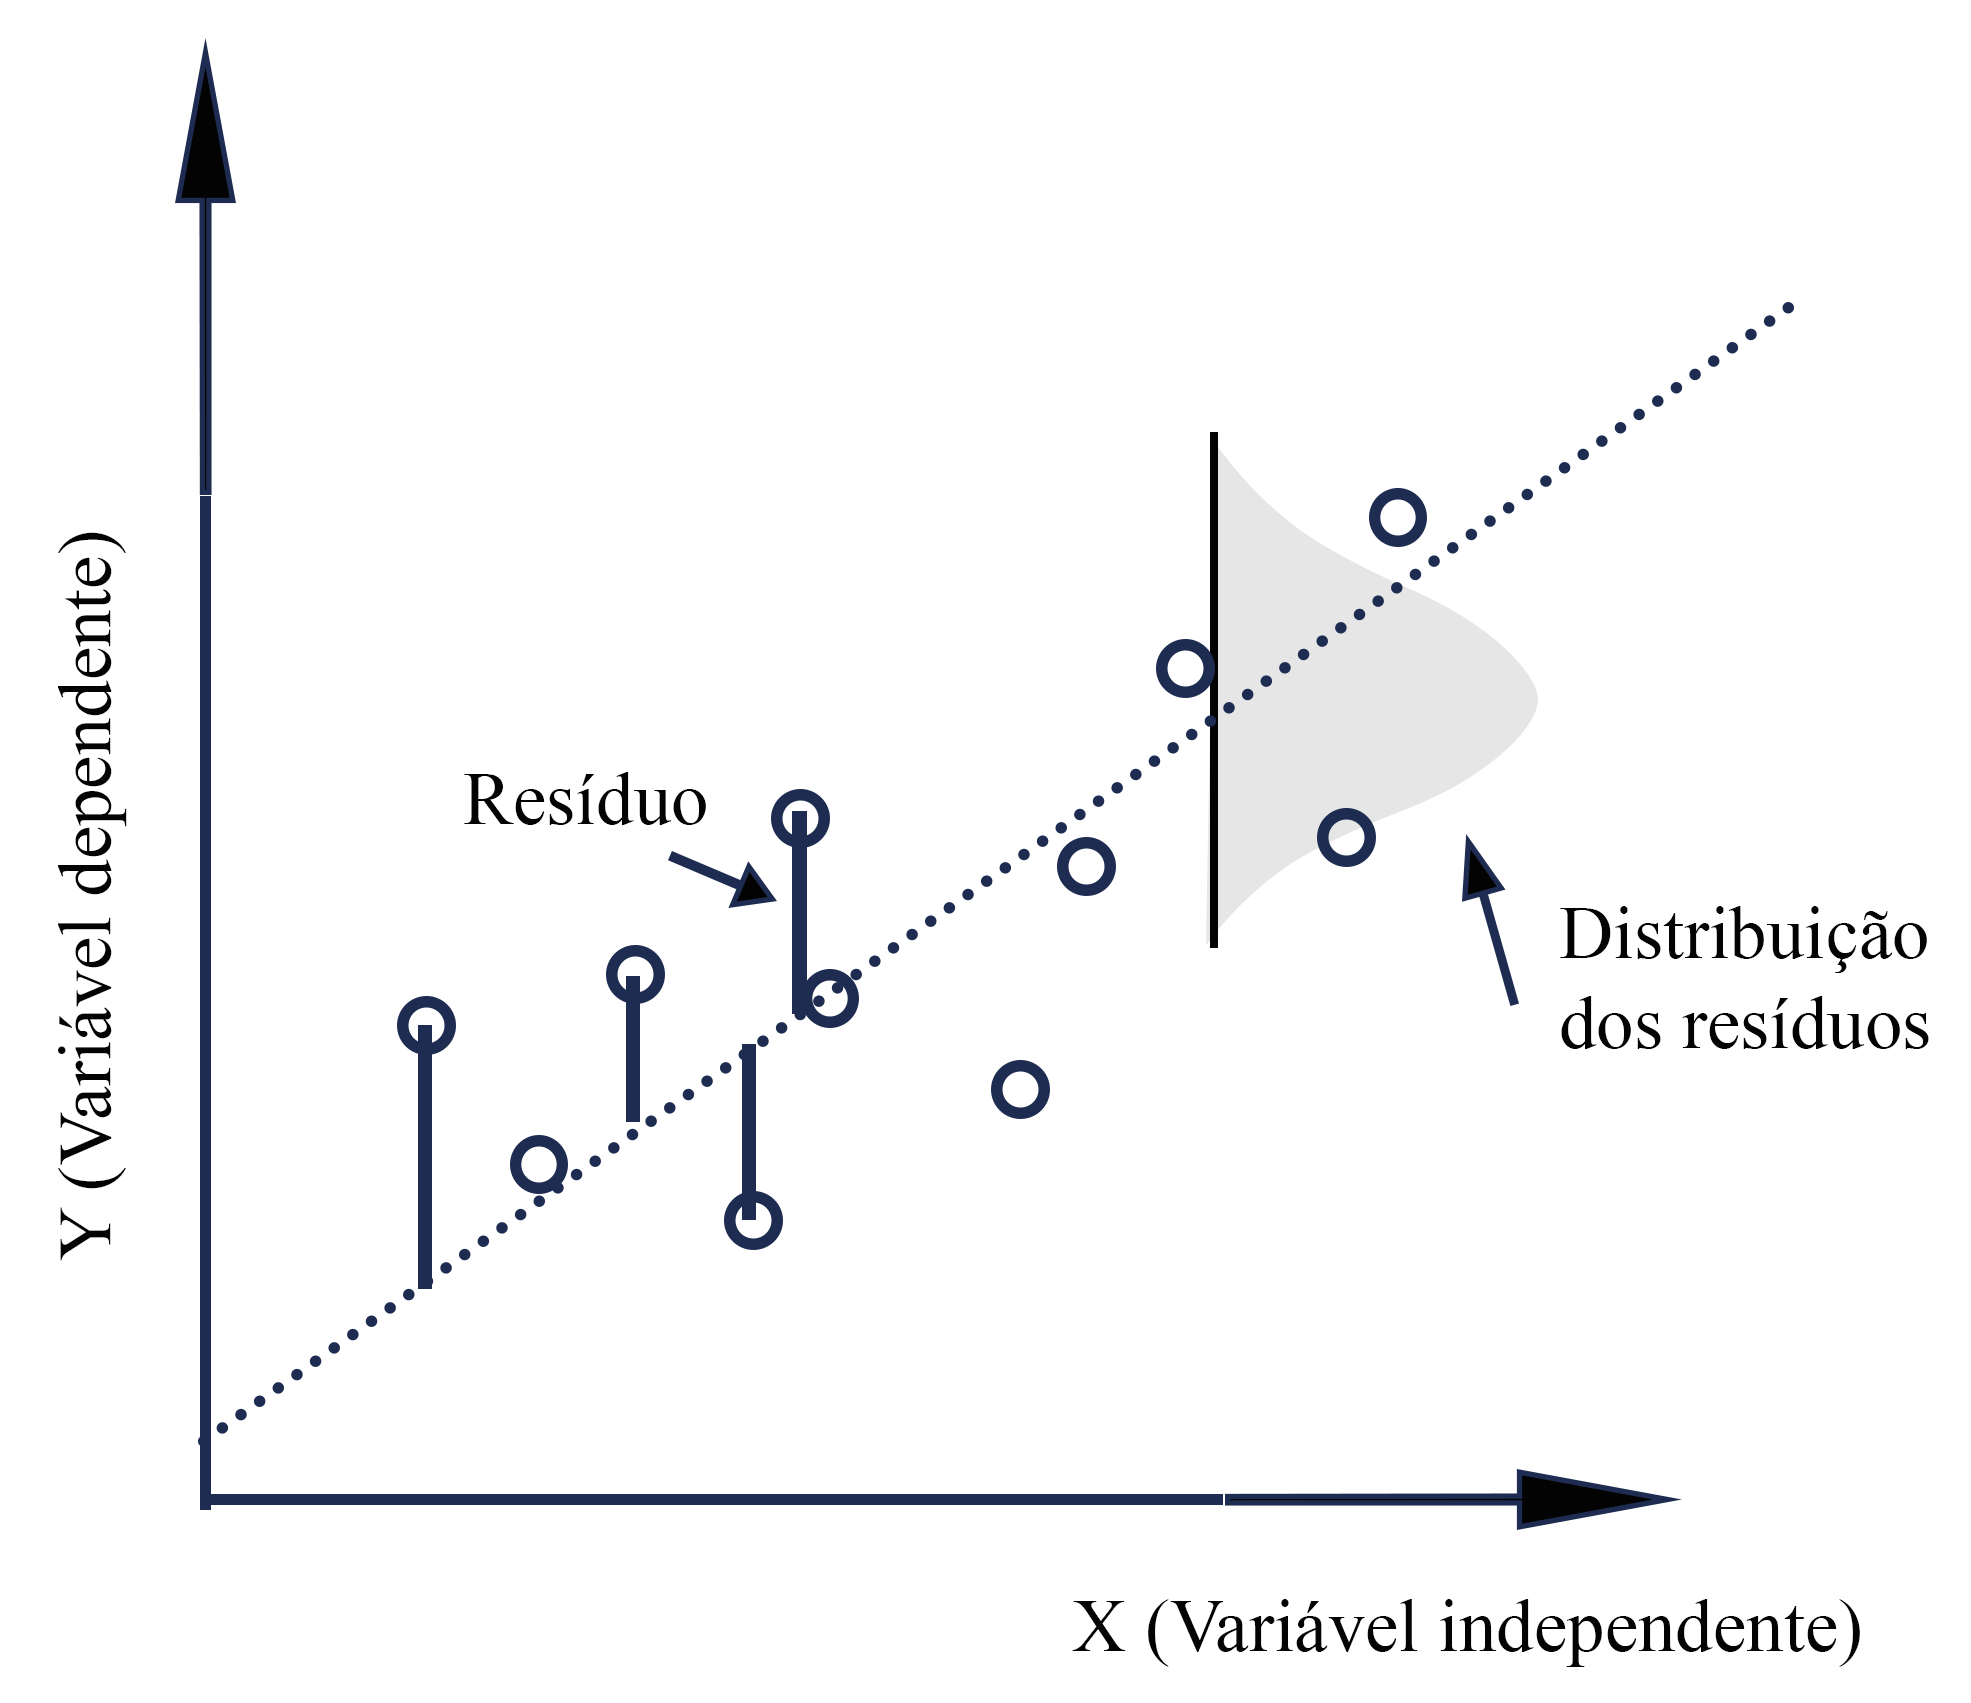
\includegraphics[scale=0.8]{regress_expl.png}	
   	\caption{Explicação da regressão linear entre a variável independente X e a variável dependente Y. Barras verticais representando o os desvios das amostras com o valor médio. }
   	\label{scatter_expl}
   \end{figure}
   
 \section{Intervalo de segurança para a regressão linear}
 
 Ao denotarmos a regressão linear entre duas variáveis é interessante estipular um intervalo de segurança para este valor, lembrando que a média  nunca pode estar sozinha de uma outra estatística para que agregue mais informações sobre as amostras. A fórmula \eqref{intervalo_seguranca} demonstra como podem ser calculadas as bandas de incerteza da regressão. 
 
 \begin{equation}\label{intervalo_seguranca}
	 Y_{i} \pm  t^{*}_{n-2} s_{y} \sqrt{\frac{1}{n}+\frac{(x_{i}-\bar{x})^2}{(n-1)s^2_{x}}}
 \end{equation}
 
 Em que $x_{i}$ é o valor da variável X a ser estimada a curva da banda, $t^*_{n-2}$ é o valor da distribuição de t-student para um grau de liberdade igual a n-2 e $s_{y}$ pode ser demonstrado segundo a equação \eqref{intervalo_seguranca2}
 
  \begin{equation}\label{intervalo_seguranca2}
  s_{y} = \sqrt{\frac{\sum_{i}(y_{i}-Y_{i})^2}{n-2}}
  \end{equation}
   
  Em que $y_{i}$ é o valor da coordenada y para um ponto amostral i. Ou seja $s_{y}$ é o valor do desvio padrão entre os valores amostrais e os valores médios estimados pela regressão. 
  
  A figura \eqref{inter_seg} demonstra o intervalo de segurança para o valor regredido. 
  
  \begin{figure}[H]
  	\centering
  	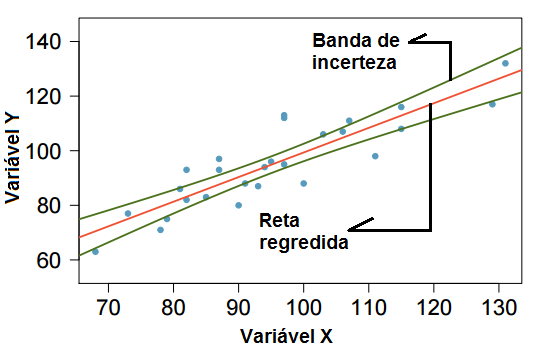
\includegraphics[scale=0.8]{banda_incerteza.png}	
  	\caption{Demonstração do intervalo de confiança para a regressão linear. Banda de incerteza adicionada como limite inferior e superior dado pela equação \eqref{intervalo_seguranca} }
  	\label{inter_seg}
  \end{figure}
  
  Nota-se que as bandas apesar de acompanharem o valor de regressão linear não são retas, apresentado um maior estreitamento na região mediana da dispersão. 
  
 \section{Regressão linear múltipla}
 
 O modelo de regressão linear múltipla é um caso extendido da regressão linear simples para múltiplas variáveis. Neste caso temos um conjunto de n variáveis independentes e n variáveis dependentes, tais que para cada variável dependente temos uma combinação linear de variáveis independentes.
 
  \begin{equation}\label{eq1:Metodo_dos_minimos_quad}
  Y_{i}^{1} = \beta_{0} + \beta_{1} X_{i}^{1} + \beta_{2} X_{i}^{2} + \beta_{3} X_{i}^{3} ...\beta_{n} X_{i}^{n} + \epsilon_{i}
  \end{equation} 
  
  Isso resulta em uma matriz de valores correlacionados como demonstrado na equação \eqref{eq1:Metodo_dos_minimos_quad_matriz}
  
  
   \begin{equation}\label{eq1:Metodo_dos_minimos_quad_matriz}
   \left\|\begin{array}{rcr}
       y_{1}\\
       y_{2}\\
       ...\\
       y_{n}
   \end{array}\right| = 
   \left\| \begin{array}{cccc}
	   x_{1}^{1}&x_{2}^{1}&....&x_{n}^{1}\\
	   x_{1}^{2}&x_{2}^{2}&....&x_{n}^{2}\\
	   ....&....&....& ....\\
	   x_{1}^{n}&x_{1}^{n}&....&x_{1}^{n}\\ 
   \end{array} \right|  
   \left\|\begin{array}{rcr}
   \beta_{1}\\
   \beta_{2}\\
   ...\\
   \beta_{n}
   \end{array}\right| 
   +   
   \left\|\begin{array}{rcr}
   \epsilon_{1}\\
   \epsilon_{2}\\
   ...\\
   \epsilon_{n}
   \end{array}\right| 
   \end{equation} 
 
 O erro quadrádico pode então ser determinado por \eqref{erroquad}
 
 \begin{equation}\label{erroquad}
 \sum_{i} \epsilon_{i}^2 = \sum_{i} \left( Y_{i} - \beta_{0} - \beta_{1} X_{i}^{1} - \beta_{2} X_{i}^{2} - ... - \beta_{n}X{i}^{n}\right) ^2 
 \end{equation}
 
 O resultado dos coeficientes $\beta$ podem ser encontrados a partir de derivação parcial das equações estabelecidas. A krigagem possui similaridades muito grandes com a regressão linear múltipla, no entanto, possuí restrições de viés durante o processo de otimização realizado. 
  
  \section{Coeficiente de correlação }
  
  Vimos no capítulo 1 o conceito de covariância. Esta estatística nada mais é que uma medida da dependência linear entre duas variáveis. Variáveis conjuntas podem apresentar modelos de dependência não lineares como parabólicos, exponenciais ou hiperbólicos. No entanto, cada um destes modelos pode ser transformado em um caso simples de correspondência linear. Por esse motivo torna-se tão importante a regressão linear entre variáveis distintas.
  
  Observe a distribuição de Gates-Gaudin-Schumann comumente utilizado para demonstrar a proporção de diâmetros de partículas de minerais após a cominuição no tratamento de minérios. O modelo é exponencial demonstrado pela equação \eqref{eq3:gates-gaudin-schumann} 
  
    \begin{equation}\label{eq3:gates-gaudin-schumann}
    p(d) = \left( \frac{d}{k}\right)^m 
    \end{equation}
    
 Em que p(d) é a proporção das partículas de diâmetro médio d e k e m são constantes do problema. Tomando o logaritmo desta expressão obtemos a seguinte expressão \eqref{eq3:gates-gaudin-schumann_2}
 
  \begin{equation}\label{eq3:gates-gaudin-schumann_2}
  log(p(d)) =  m \left( log(d)-log(k)) \right)
  \end{equation}
 
Em que m e k são as variáveis desconhecidas da distribuição. Esse é um caso simples de linearização de um modelo. Alguns casos mais robustos exigem operações mais complexas, mas a grande maioria dos problemas podem ser resolvidos com linearizações simples. 

Uma forma simples de demonstrar o grau de dependência linear entre duas variáveis é utilizando o coeficiente de regressão de Pearson. Ele nada mais é que uma normalização da covariância a partir das variâncias de cada variável aleatória. Definimos o coeficiente de correlacao de Pearson segundo a equação \eqref{coeficiente_de_corr}

  \begin{equation}\label{coeficiente_de_corr}
  r = \frac{COV(X,Y)}{\sigma _{X}\sigma _{Y}}
  \end{equation}
  
 O coeficiente de correlação é uma medida que varia de -1 a 1 sendo o valor negativo igual à uma relação decrescente entre as variáveis, positivo igual uma relação crescente e 0 como independência entre as variáveis aleatórias. 
 
 Há também o chamado coeficiente de Rank. Um rank é uma varíavel que associa uma ordem para cada valor da variável aleatória. O menor valor recebe rank igual a 1, o segundo menor recebe um rank igual a 2 e assim sucessivamente até os n valores da variável aleatória. O coeficiente de Rank é então tomado como o coeficiente de correlação entre os ranks de cada variável. 
 
 O coeficiente de Rank diferentemente do coeficiente de Pearson é uma medida de tendência dos valores e não da linearidade dos valores em si. Nesse caso estamos interessados em saber apenas se existe uma correlação entre a organização das amostras sem considerar sua ordem de grandeza. Neste caso a estatística é muito menos influenciada por valores extremos. A tabela \eqref{rank_T} demonstra suscintamente como realizar o coeficiente de Rank para uma dada variável aleatória. 
 

\begin{table}[H]
	\centering
	\caption{Valores de Rank para uma variável aleatoria}
	\label{rank_T}
	\begin{tabular}{@{}ll@{}}
		\toprule
		valor da variável & Rank \\ \midrule
		50                & 4    \\
		25                & 1    \\
		60                & 5    \\
		30                & 2    \\
		45                & 3    \\ \bottomrule
	\end{tabular}
\end{table}
 
  
\section{Probabilidades condicionais e conjuntas}

Muitas vezes não estamos interessados em determinar as probabilidades ou frequências individuais de uma variável aleatória. É interessante, por exemplo, determinar qual é a frequência de um minério e que seu conteúdo tenha um determinado valor de impureza. Ou, por exemplo, qual é a frequência de acidentes e de mal uso de um EPI. Neste caso estamos trabalhando com eventos disjuntos, ou seja a interseção de valores entre variáveis aleatórias. A figura \eqref{disjuntos}
demonstra em um diagrama de Venn a interseção formada por um evento disjunto entre duas variáveis.

   \begin{figure}[H]
   	\centering
   	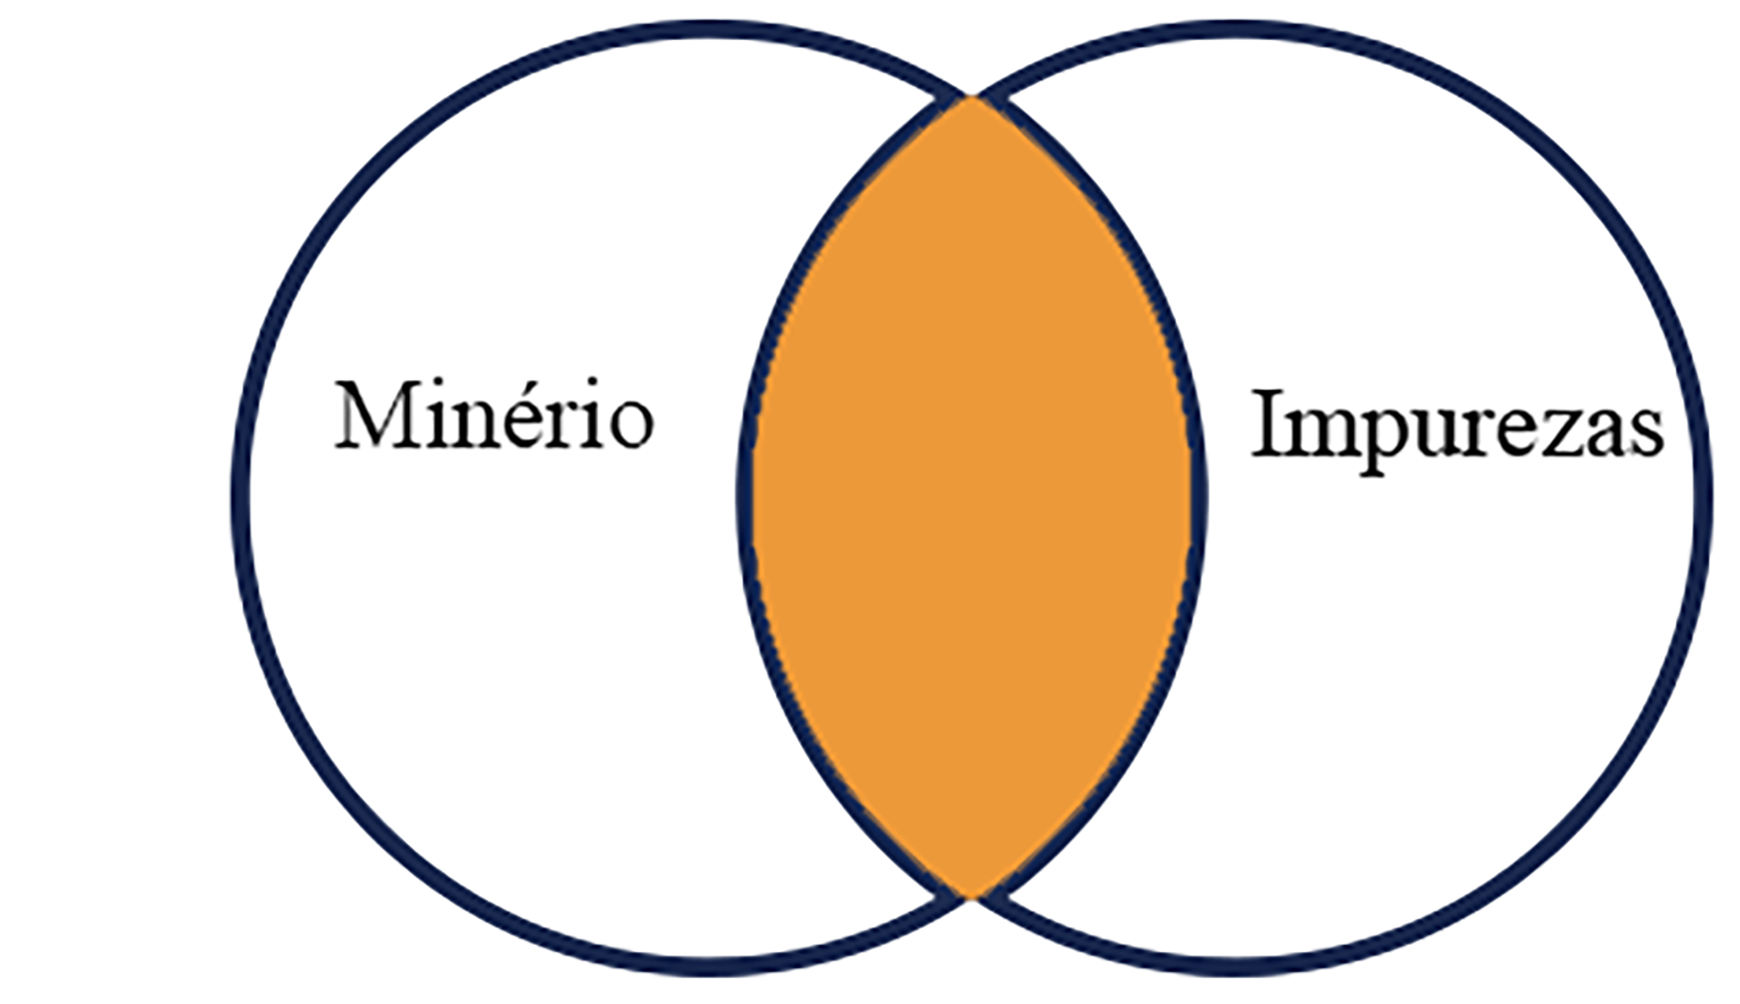
\includegraphics[scale=0.8]{DISJUNTO.png}	
   	\caption{Demonstração de eventos disjuntos entre a variável minério e impureza a partir de um diagrama de Venn.Nota-se a área laranja como sendo a interseção dos eventos }
   	\label{disjuntos}
   \end{figure}


 Observe a tabela \ref{tabela_impureza}. Notamos na coluna três o número de vezes que o minério considerado possui uma impureza maior ou igual a 0,005. Neste caso sabemos que há 2 valores em cinco em que isso ocorre. Logo a probabilidade conjunta é P(Minerio) $\bigcap$ P(Impureza $\geq$  0.005) = 2/5 = 40\%

\begin{table}[H]
\centering
\caption{Tabela da relação entre um dado minério e uma impureza}
\label{tabela_impureza}
\begin{tabular}{ccc}
	\toprule
	Minério & Impureza & Minério $\bigcap$ (Impureza \textgreater=0,005) \\ \midrule
	Sim     & 0,005    & 1                                                           \\
	Não     & 0,007    & 0                                                           \\
	Não     & 0,008    & 0                                                           \\
	Sim     & 0,006    & 1                                                           \\
	Sim     & 0,003    & 0                                                           \\ \bottomrule
\end{tabular}
\end{table} 

Da mesma forma podemos definir a probabilidade condicional como sendo a relação entre a probabilidade do evento disjunto entre as variáveis aleatórias e a probabilidade da variável aleatória. A probabilidade condicional pode ser demonstrada na figura \eqref{disjuntos2} como a relação da área laranja pela área hachurada.

\begin{figure}[H]
	\centering
	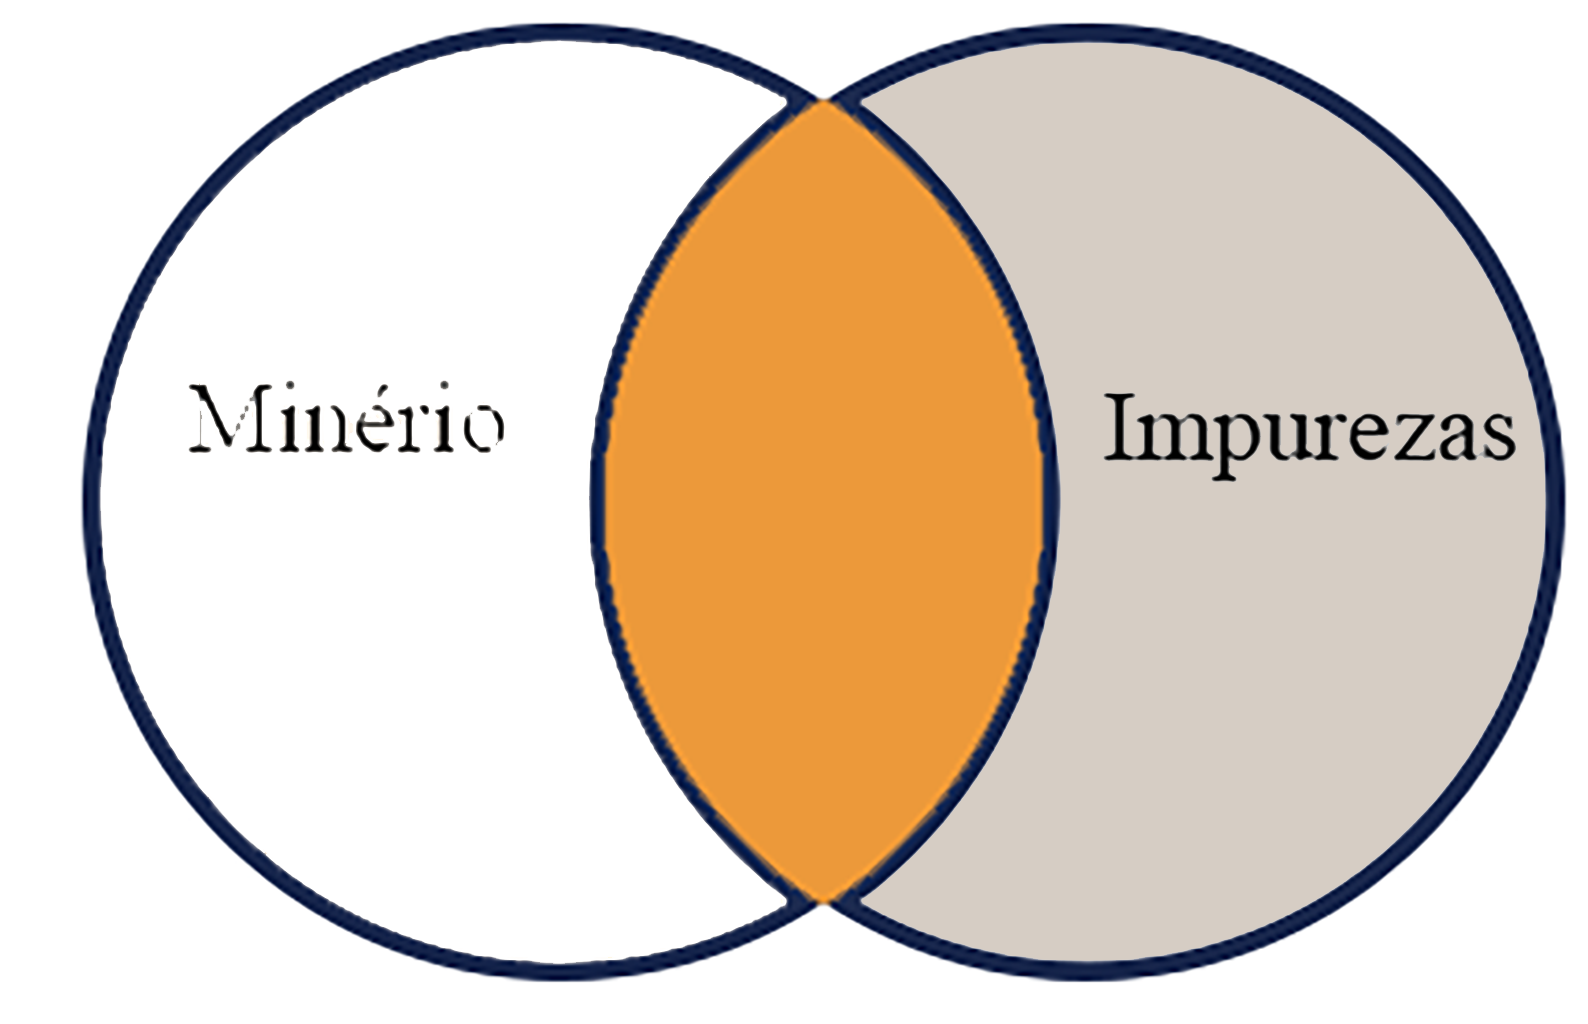
\includegraphics[scale=0.8]{DISJUNTO_2.png}	
	\caption{Demonstração da probabilidade condicional entre a variável minério e impureza a partir de um diagrama de Venn.Nota-se a área laranja como sendo a interseção dos eventos disjuntos. A probabilidade condicional é a relação entre a área laranja pela área hachurada. }
	\label{disjuntos2}
\end{figure} 
   
Na tabela \ref{tabela_impureza} podemos calcular a probabilidade condicional tal como  $P(M=Sim | I \geq 0,005) = \frac{2/5}{3/5} = 67\%$. Ou seja, dado que encontremos um minério, a chance de ele possuir valor acima de impureza acima de 0,005 é de $67\%$

A figura \eqref{hist_cond} demonstra como pode ser calculado o histograma marginal de uma variável a partir de um gráfico de dispersão. Todos os valores abaixo de 5 da variável Y são selecionados para realizar o  histograma. 

\begin{figure}[H]
	\centering
	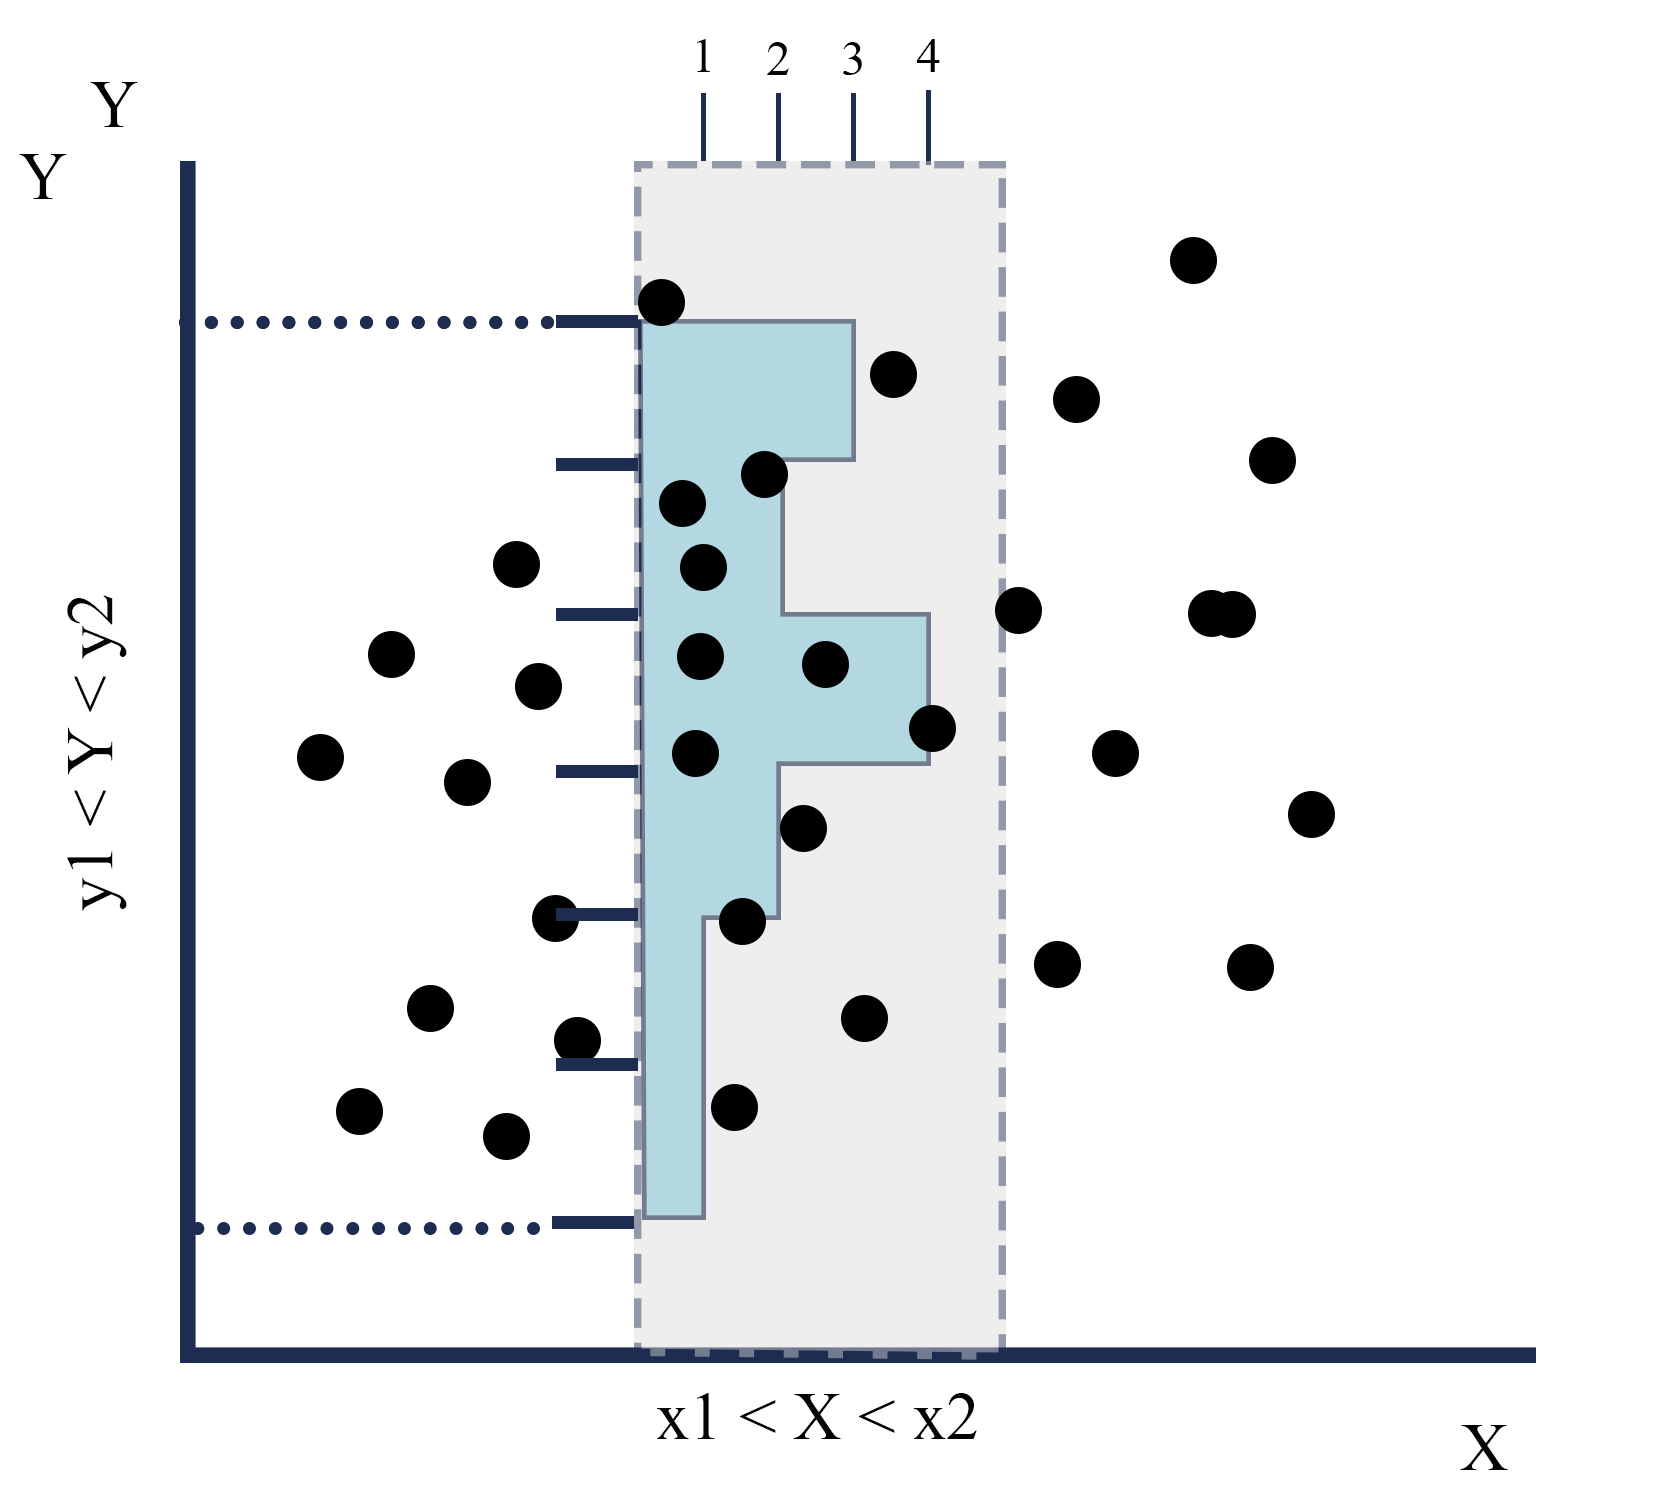
\includegraphics[scale=0.7]{hist_cond.png}	
	\caption{Histograma condicional criado a partir de um gráfico de dispersão. Valores abaixo de 5 da variável Y são selecionados para realizar o histograma da direita.  }
	\label{hist_cond}
\end{figure}

\section{Teste qui-quadrado para independência entre variáveis}

Em alguns casos é importante verificarmos se determinado conjunto de variáveis é independente. No âmbito da geoestatística, variáveis estimadas que são independentes produzem o mesmo resultado que variáveis estimadas em conjunto. Observe a tabela \eqref{tabela_pocos}. A tabela mostra o nível de 4 poços controlados durante 4 dias seguintes. Deseja-se saber se os poços são dependentes e interconectados. 

\begin{table}[H]
	\centering
	\caption{Nivel de quatro poços controlados por dia}
	\label{tabela_pocos}
	\begin{tabular}{l|l|l|l|l|l|}
		\cline{2-6}
		& poço 1 & poço 2 & poço 3 & poço 4 & soma \\ \hline
		\multicolumn{1}{|l|}{dia 1} & 10     & 30     & 20     & 40     & 100  \\ \hline
		\multicolumn{1}{|l|}{dia 2} & 20     & 20     & 25     & 35     & 100  \\ \hline
		\multicolumn{1}{|l|}{dia 3} & 5      & 10     & 20     & 30     & 55   \\ \hline
		\multicolumn{1}{|l|}{dia 4} & 20     & 30     & 30     & 30     & 110  \\ \hline
		\multicolumn{1}{|l|}{soma}  & 55     & 90     & 95     & 135    & 375  \\ \hline
	\end{tabular}
\end{table}

O teste para a verificação de dependência é o qui-quadrado, sendo expresso equação:
   
\begin{equation}\label{quiquadrado}
\chi ^2 = \sum_{i=1}^{n}\sum_{j=1}^{n} \frac{(O_{i,j}-E_{i,j})^2}{E_{i,j}}
\end{equation}

Em que $E_{i,j}$ são as frequências esperadas para cada uma das observações $O_{i,j}$ :

\begin{equation}\label{ezinho}
E_{i,j} = \frac{\left( \sum_{i=1}^{n}O_{i,j}\right) \left( \sum_{i=j}^{n}O_{i,j}\right)}{\sum_{i=1}^{n}\sum_{j=1}^{n} O_{i,j}}
\end{equation}

O valor da distribuição qui quadrado deve ser avaliado segundo o grau de liberdade do conjunto de amostras. A ideia de graus de liberdade na estatística está relacionado com o número de amostras menos o número de parâmetros estimados. Neste caso o número de graus de liberdade pode ser calculado como o número de colunas da tabela vezes o número de linhas menos um. Logo o grau de liberdade da tabela deste problema é $4*(4-1) =12$

Consideramos como hipótese nula no teste qui-quadrado para independência das amostras que as frequências esperadas não são diferentes das frequências observadas, logo as amostras são dependentes. Como hipótese alternativa consideramos que as frequências esperadas são diferentes das observadas, logo as amostras são independentes.

\begin{enumerate}
	\item Se o valor de $\chi^2$ calculado for $\geq$ ao valor tabelado para um nível de significância, então podemos considerar a hipótese nula rejeitada e as amostras são idependentes
	\item Se o valor de $\chi^2$ calculado for $\leq$ ao valor tabelado para um nível de significância, então falhamos em descartar a hipótese nula e podemos considerar as amostras dependentes. 
\end{enumerate}

Realizando os cálculos para a tabela acima encontramos um valor de $\chi^2= 17,88$. O valor da distribuição qui-quadrado para um grau de liberdade igual a 12 e um nível de significância de 5\% é de 5,22. Como o valor calculado é maior que o tabelado descartamos a hipótese nula de dependência e a as amostras são independentes. 

O teste qui-quadrado é flexível e pode ser utilizado em diversas situações em que se deseja comparar as proporções de diferentes variáveis ou modelos. Pode ser utilizado juntamente com o valor p de gráficos de probabilidade para determinar o ajuste de distribuições. 